
% BEGIN COPY
\DeclareRobustCommand{\LFtok}[1]{\mbox{\texttt{\textbf{[#1]}}}}
\section{LoopFill Decoding}
\label{sec:loopfill}

LoopFill builds a single draft tree from two sources. As in
SuffixDecoding~\cite{oliaro2025suffixdecodingextremespeculativedecoding},
suffix matches supply continuations that occurred in earlier text.
As in LoopSpec~\cite{cho2026loopspecpipelinedselfspeculativedecoding},
the model can propose a next token before the current position finishes
all $T$ loops. A suffix match can extend a token proposed by an early
loop, and an early prediction can extend a token retrieved from the
suffix tree.

Each additional draft position consumes model computation on every
loop it runs. When many requests share a device, spending that
computation on branches that will be discarded can lower output
throughput. For candidates from either source, we estimate how often
they match the full-depth greedy next token on calibration prompts.
LoopFill combines these estimates along each path and processes a draft
node only while its path score exceeds a threshold. Only the full-depth
prediction at the verified prefix determines which token the decoder
appends.

Figure~\ref{fig:loopfill-trees} follows the example in
Figure~\ref{fig:four-decoders}. With $T=3$, LoopFill produces the five
output tokens in five loop steps. Greedy decoding takes fifteen.

\begin{figure}[t]
  \centering
  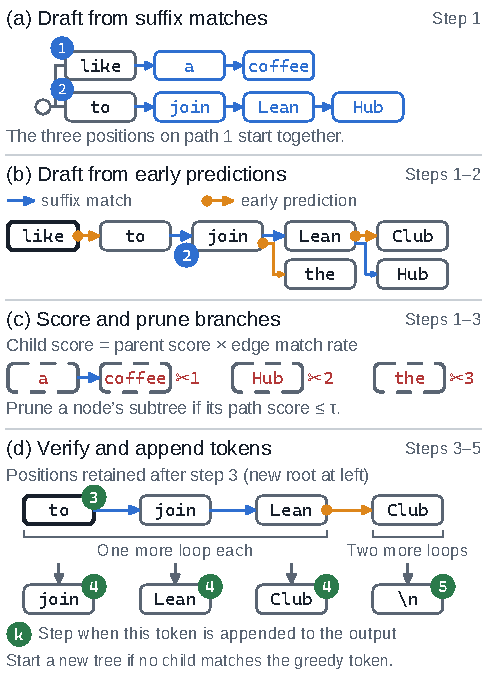
\includegraphics[width=0.65\columnwidth]{figures/02_tree.pdf}
  \caption{\textbf{LoopFill decoding with three loops per position.}
    (a)~A suffix match at \LFtok{like} proposes \LFtok{a} \LFtok{coffee}.
    (b)~Both early-loop predictions (orange edges) and suffix-tree
    matches (blue edges) add tokens to the same draft tree. The first
    loop at \LFtok{like} adds \LFtok{to}, and a suffix match supplies
    the next edge from \LFtok{to} to \LFtok{join}.
    (c)~Pruning \LFtok{a} at step~1 also removes \LFtok{coffee}.
    (d)~After the decoder verifies \LFtok{to} at step~3, the retained
    positions predict the tokens shown below them. Green badges give
    the step when each output token is appended.}
  \label{fig:loopfill-trees}
\end{figure}

\paragraph{Growing the draft tree.}
The suffix tree indexes the prompt, the verified output so far,
and outputs from earlier requests. A query matches a suffix of a given
prefix against the index and returns the continuations that followed the
match. The draft tree stores the candidates that LoopFill will
process for the current request. Its root represents the verified prefix
$x$. A node $u$ represents
$x$ followed by the draft tokens on the path to that node. A child
$ua$ extends $u$ by one candidate token $a$.

Each node processes the last token of its prefix to predict the token
after that prefix. Attention at the node uses only the verified
prefix and the tokens on its own path. In Figure~\ref{fig:loopfill-trees}(a),
a suffix match lets \LFtok{a} and \LFtok{coffee} start their first loop
alongside \LFtok{like}. Each step advances every unfinished
position by one loop. The decoder reads the next-token distribution at $u$
after $d_1$ loops and again if $u$ reaches $d_2$ loops ($d_1<d_2<T$).
We call each readout a shallow prediction. The candidates for
the next position are the top eight
tokens in that distribution together with the tokens labeling the
existing children of $u$. When the decoder admits a new child $ua$ from
a shallow prediction at $u$, it queries the suffix index with the prefix
ending at $ua$. Nodes admitted during one step can start their first
loop in the next step.

Figure~\ref{fig:loopfill-trees}(b) shows how the two sources extend the
same branch. The first loop at \LFtok{like} proposes \LFtok{to}.
Querying the suffix tree with the prefix ending in \LFtok{to} adds
the path \LFtok{join} \LFtok{Lean} \LFtok{Hub}. All four positions
start in step~2. The first loop at \LFtok{Lean} then proposes
\LFtok{Club} as another child of \LFtok{Lean}.

\paragraph{Calibrating and pruning drafts.}
Computing a node is useful for the output only if every token on its
path agrees with greedy decoding. For each edge from $u$ to $ua$, we
estimate the probability $\hat q(a\mid u)$ that the greedy next token
after $u$ is $a$, conditional on $u$ being on the greedy path. Before
decoding, we generate greedy outputs for a set of calibration prompts.
At prefixes on those outputs we group candidates by the features below
and record the fraction in each group that match the full-depth greedy
next token. For suffix candidates we collect these observations at the
prefixes where the decoder actually queries the suffix index.

For a suffix proposal, the features $m$ record the suffix-match
length, the relative frequency of $a$ among continuations, whether $u$ has other
children, and the depth of $u$ in the draft tree. Let $b$ indicate
whether the suffix tree proposed $a$. Let $r_i$ and $p_i$ be the rank
and probability of $a$ in the shallow prediction at loop $d_i$.
A token outside the top eight receives a reserved rank and $p_i=0$.
The decoder updates the edge estimate using fixed match-rate tables $M$.
\[
\hat q(a\mid u)\gets
\left\{\begin{array}{@{}l@{\quad}l@{}}
 M_{\mathrm{suf}}(m)  & \mbox{on a suffix proposal},\\
 M_1(r_1,p_1,b)       & \mbox{after $d_1$ loops},\\
 M_2(r_1,r_2,p_2,b)   & \mbox{after $d_2$ loops}.
\end{array}\right.
\]
Each update replaces the previous estimate for that edge. The root
score is $s(x)=1$, and a child's path score is
$s(ua)=s(u)\,\hat q(a\mid u)$. For example, edge estimates of $0.8$
for \LFtok{to} after the root and $0.5$ for \LFtok{join} after
\LFtok{to} give the path \LFtok{to} \LFtok{join} a score of $0.4$.

The decoder keeps a draft node only while its path score exceeds
$\tau$. When an edge estimate changes, the decoder recomputes the
scores of all paths through that edge. When a node's score falls to
$\tau$ or below, the decoder removes that node and its descendants.
In Figure~\ref{fig:loopfill-trees}(c), the score for \LFtok{a} falls to
$\tau$ or below at step~1, so pruning \LFtok{a} also removes its child
\LFtok{coffee}.

To select $\tau$ on development prompts, we count both the sequential
loop steps per output token and the number of positions processed per
output token, counting a position once for each loop it runs.
A lower threshold can save steps
by starting correct positions earlier. A higher threshold can reduce
the work spent on incorrect branches. We use $\tau=0.01$ for the
low-load setting and $\tau=0.1$ when limiting draft computation takes
priority.

\paragraph{Verifying tokens and reusing completed loops.}
When the root for $x$ finishes all $T$ loops, the decoder takes the
greedy next token $a$ at that root, appends $a$ to the output, and
adds $a$ to the suffix index. If the root has a child $xa$, the
decoder makes that child the new root with score one, keeps the
child's subtree and its completed loops, and discards the old root's
other branches. From this new root the decoder recomputes path scores
and queries the suffix index for continuations of $xa$. If no child
matches $a$, the decoder starts a
new draft tree at $xa$. Every emitted token is therefore the full-depth
greedy prediction at its verified prefix.

A new root that has already finished all $T$ loops can supply the next
output token in the same step. In Figure~\ref{fig:loopfill-trees}(d),
the final prediction at the position processing \LFtok{like} is
\LFtok{to} in step~3. By then \LFtok{to}, \LFtok{join}, and
\LFtok{Lean} have each completed two loops. In step~4 those positions
finish together, and the decoder appends their predictions
\LFtok{join}, \LFtok{Lean}, and \LFtok{Club} in order. In step~5 the position
processing \LFtok{Club} finishes its last loop and predicts
\LFtok{\textbackslash n}. Algorithm~\ref{alg:loopfill} summarizes
one loop step.

% Share the host's algorithm counter when its algorithm package is loaded.
\ifcsname c@algorithm\endcsname\else\newcounter{algorithm}\fi
\par\medskip
\noindent\begin{minipage}{\linewidth}
\refstepcounter{algorithm}\label{alg:loopfill}
\hrule\smallskip
\textbf{Algorithm \thealgorithm.\quad LoopFill decoding}\par
\smallskip
\textbf{Start.} Create a draft tree with verified prefix $x$ as its root
and $s(x)=1$. Add suffix continuations one token at a time while their
path scores exceed $\tau$.\par
\smallskip
\textbf{Repeat} for each loop step\par
{\leftskip=1em\relax
Advance every unfinished node by one loop.\par
\textbf{While} the root for $x$ has completed $T$ loops\par
{\leftskip=2em\relax
Let $a$ be the root's greedy next token. Append $a$ to the output and
add $a$ to the suffix index. Stop if the output is complete.\par
Set $x\gets xa$. If the tree has no node for the updated prefix $x$,
return to \textbf{Start}.\par
Make that node the root with $s(x)=1$. Retain its subtree and completed
loops, recompute path scores from $x$, and add suffix drafts from $x$.\par}
\textbf{For each} surviving node $u$ that just completed $d_1$ or $d_2$ loops\par
{\leftskip=2em\relax
Score the existing children of $u$ and the top eight next tokens in its
shallow prediction. Keep a candidate $ua$ only if $s(ua)>\tau$.
Otherwise discard $ua$ and any descendants.\par
Add suffix drafts from each newly added child.\par}}
\smallskip\hrule
\end{minipage}\par
% END COPY